% % % % % % % % % % % % % % % % % % % % % % % % % % % % % % % % % % % % % % % % %
% INTRO
% % % % % % % % % % % % % % % % % % % % % % % % % % % % % % % % % % % % % % % % %
\section{Time box 6}
\listoftodos
\subsection{Time box planning}

\begin{figure}[H]
	\begin{centering}
		\missingfigure{Updated timebox figure}
		%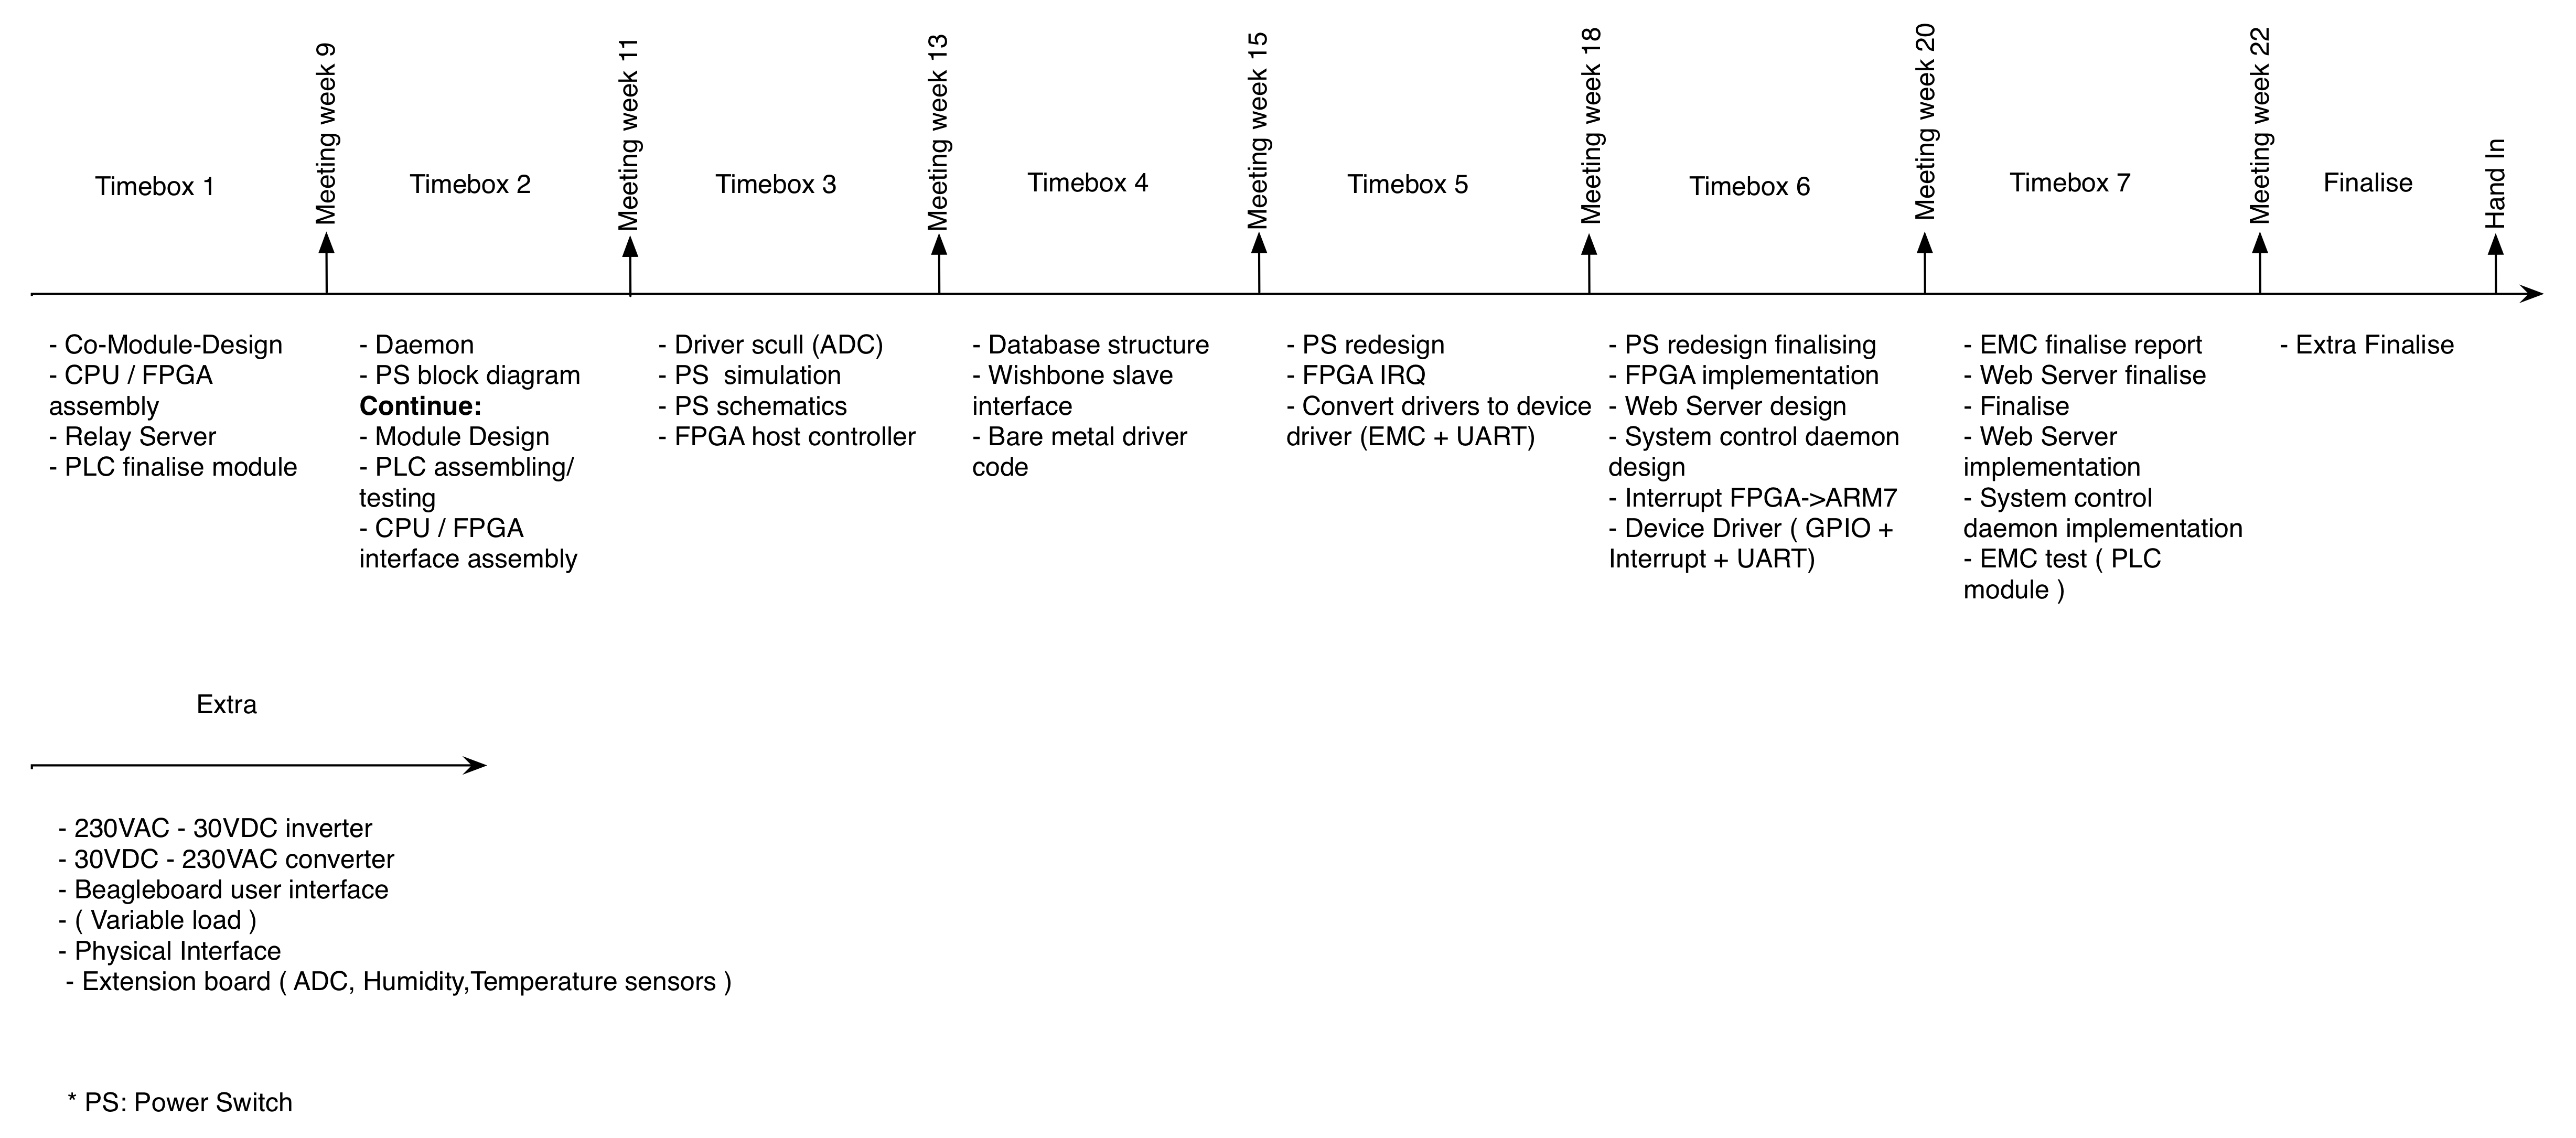
\includegraphics[width=1.0\textwidth]{images/tb_r5.png}
		%\caption{Updated time-box}
	\end{centering}
\end{figure}

\subsubsection{Work to be done in this time box}
\todo[inline]{Update List}
\begin{itemize}
	\item Switch interrupt
	\begin{itemize}
		\item debouncer
		\item Interrupt
	\end{itemize}
	\item Jesus thing
		\begin{itemize}
			\item sub thing
		\end{itemize}
	\item UART Device driver
	\begin{itemize}
		\item Improvement on the driver made in last timebox
	\end{itemize}
\end{itemize}

\paragraph{Description:}
\todo[inline]{Update Description}
\begin{description}
	\item[Switch interrupt] In order to send data to the interrupt register, an interrupt output for the switch block has to be implemented, and the switches has to be debounced, to secure that the interrupt data is send only once.
	\item[Jesus thing]
	\item[UART Device driver] Implementation of input/output control and interrupt handling in the UART device driver made in time box 5.
\end{description}

\subsubsection{Time planning}

\begin{table}[H]
\centering
	\todo[inline]{Update Time}
	\begin{tabular}{|l|c|c|c|c|c|}
		\hline
		~			& Switch interrupt			& Jesus thing		& UART improvements	\\ \hline
		Estimation	& 12					& xx				& 5				\\
		Actual		& 20					& xx				& 15			\\
		Developer	& Theis					& Paulo				& Dennis		\\
		\hline
	\end{tabular}
	\caption{Estimation and actual time used on the project}
\end{table}

% % % % % % % % % % % % % % % % % % % % % % % % % % % % % % % % % % % % % % % % %
% % % % % % % % % % % % % % % % % % % % % % % % % % % % % % % % % % % % % % % % %
% Scaling the project due to limited time.
% % % % % % % % % % % % % % % % % % % % % % % % % % % % % % % % % % % % % % % % %
\subsection{Project scaling}
What have been downscaled in the project in order to make something to work. 





% % % % % % % % % % % % % % % % % % % % % % % % % % % % % % % % % % % % % % % % %
% % % % % % % % % % % % % % % % % % % % % % % % % % % % % % % % % % % % % % % % %
% Theis Thing
% % % % % % % % % % % % % % % % % % % % % % % % % % % % % % % % % % % % % % % % %
\subsection{Switch interrupt - Theis}
%			Intro
%					verification specification
%					deployment specification
%
This part is, together with the interrupt register from earlier timebox a way to tune performance in reading and writing between the Spartan 6 and the LPC2478.
\subsubsection{Analysis}
%			Analysis
%
%                Refactored block diagram
%                Refactored class diagram
%                Detailed use cases
%                User interface specification
%                System interface specification
%                Dimensioning specification 
%
The interrupt block in the Spartan 6 is the switch block. The switch block needs to be redesign in order to get an interrupt output to the interrupt register, the switches also needs to be debounced, to prevent it from sending the same interrupt data more than once. Two output is added to the switch block, one single bit for interrupt indication and a 7 bit vector for the data to the interrupt register. Inside the block a finite state machine is made for denouncing the switches. Below the redesigned switch block is shown.

\begin{figure}[H]
	\begin{centering}
		%\missingfigure{Updated timebox figure}
		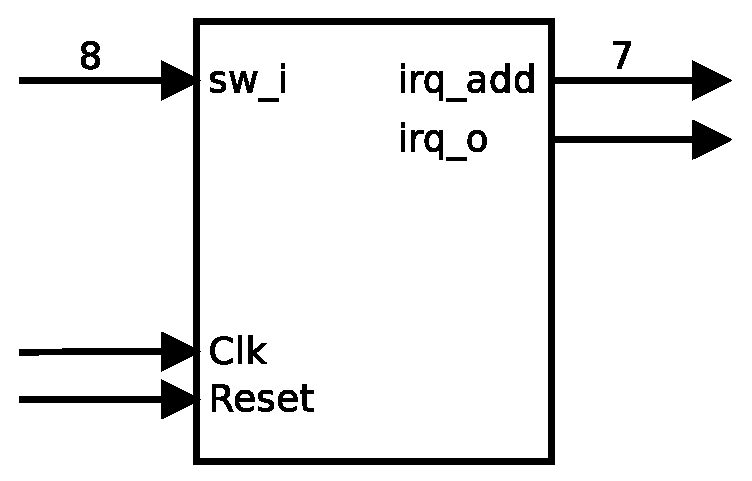
\includegraphics[width=0.3\textwidth]{images/tb6_switchblock.eps}
		\caption{Updated switch block}
	\end{centering}
\end{figure}


\subsubsection{Design}
%       	 Design
%
%                UML/SysML deployment view(s)
%                Mechanical specifications and dimensioning
%                HW module specification per block
%                UML SW deployment view
%                Class specification
%                Refactored class diagram
%                Use case scenarios specifications
%                Sequence diagrams
%
Because of switch bounce, the block needs to take care of this. Below a picture of switch bouncing is shown. The problem is every time the signal goes high the switch block will send data to the interrupt register, to prevent this the block compare a delayed input signal to the present signal, and first when the signal is stable, the system will react on the input.

\begin{figure}[H]
	\begin{centering}
		%\missingfigure{Updated timebox figure}
		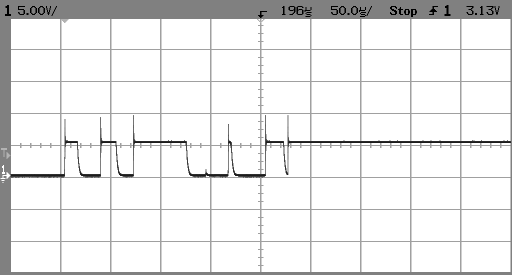
\includegraphics[width=0.5\textwidth]{images/tb6_bounce.png}
		\caption{Switch bouncing}
	\end{centering}
\end{figure}

To debounce the switch a state machine for the switch block is made. This diagram is shown below. The start box set the start output signal to the input signal. The interrupt signal is set high in the OUT0 state, and low again in the IDLE state after the "q2" delay. This is done to have the interrupt signal high enough time for the interrupt register to save the data. The "q1" delay is used to compare the input signal with the output signal in order to capture changes on the 8 switches.

\begin{figure}[H]
	\begin{centering}
		%\missingfigure{Updated timebox figure}
		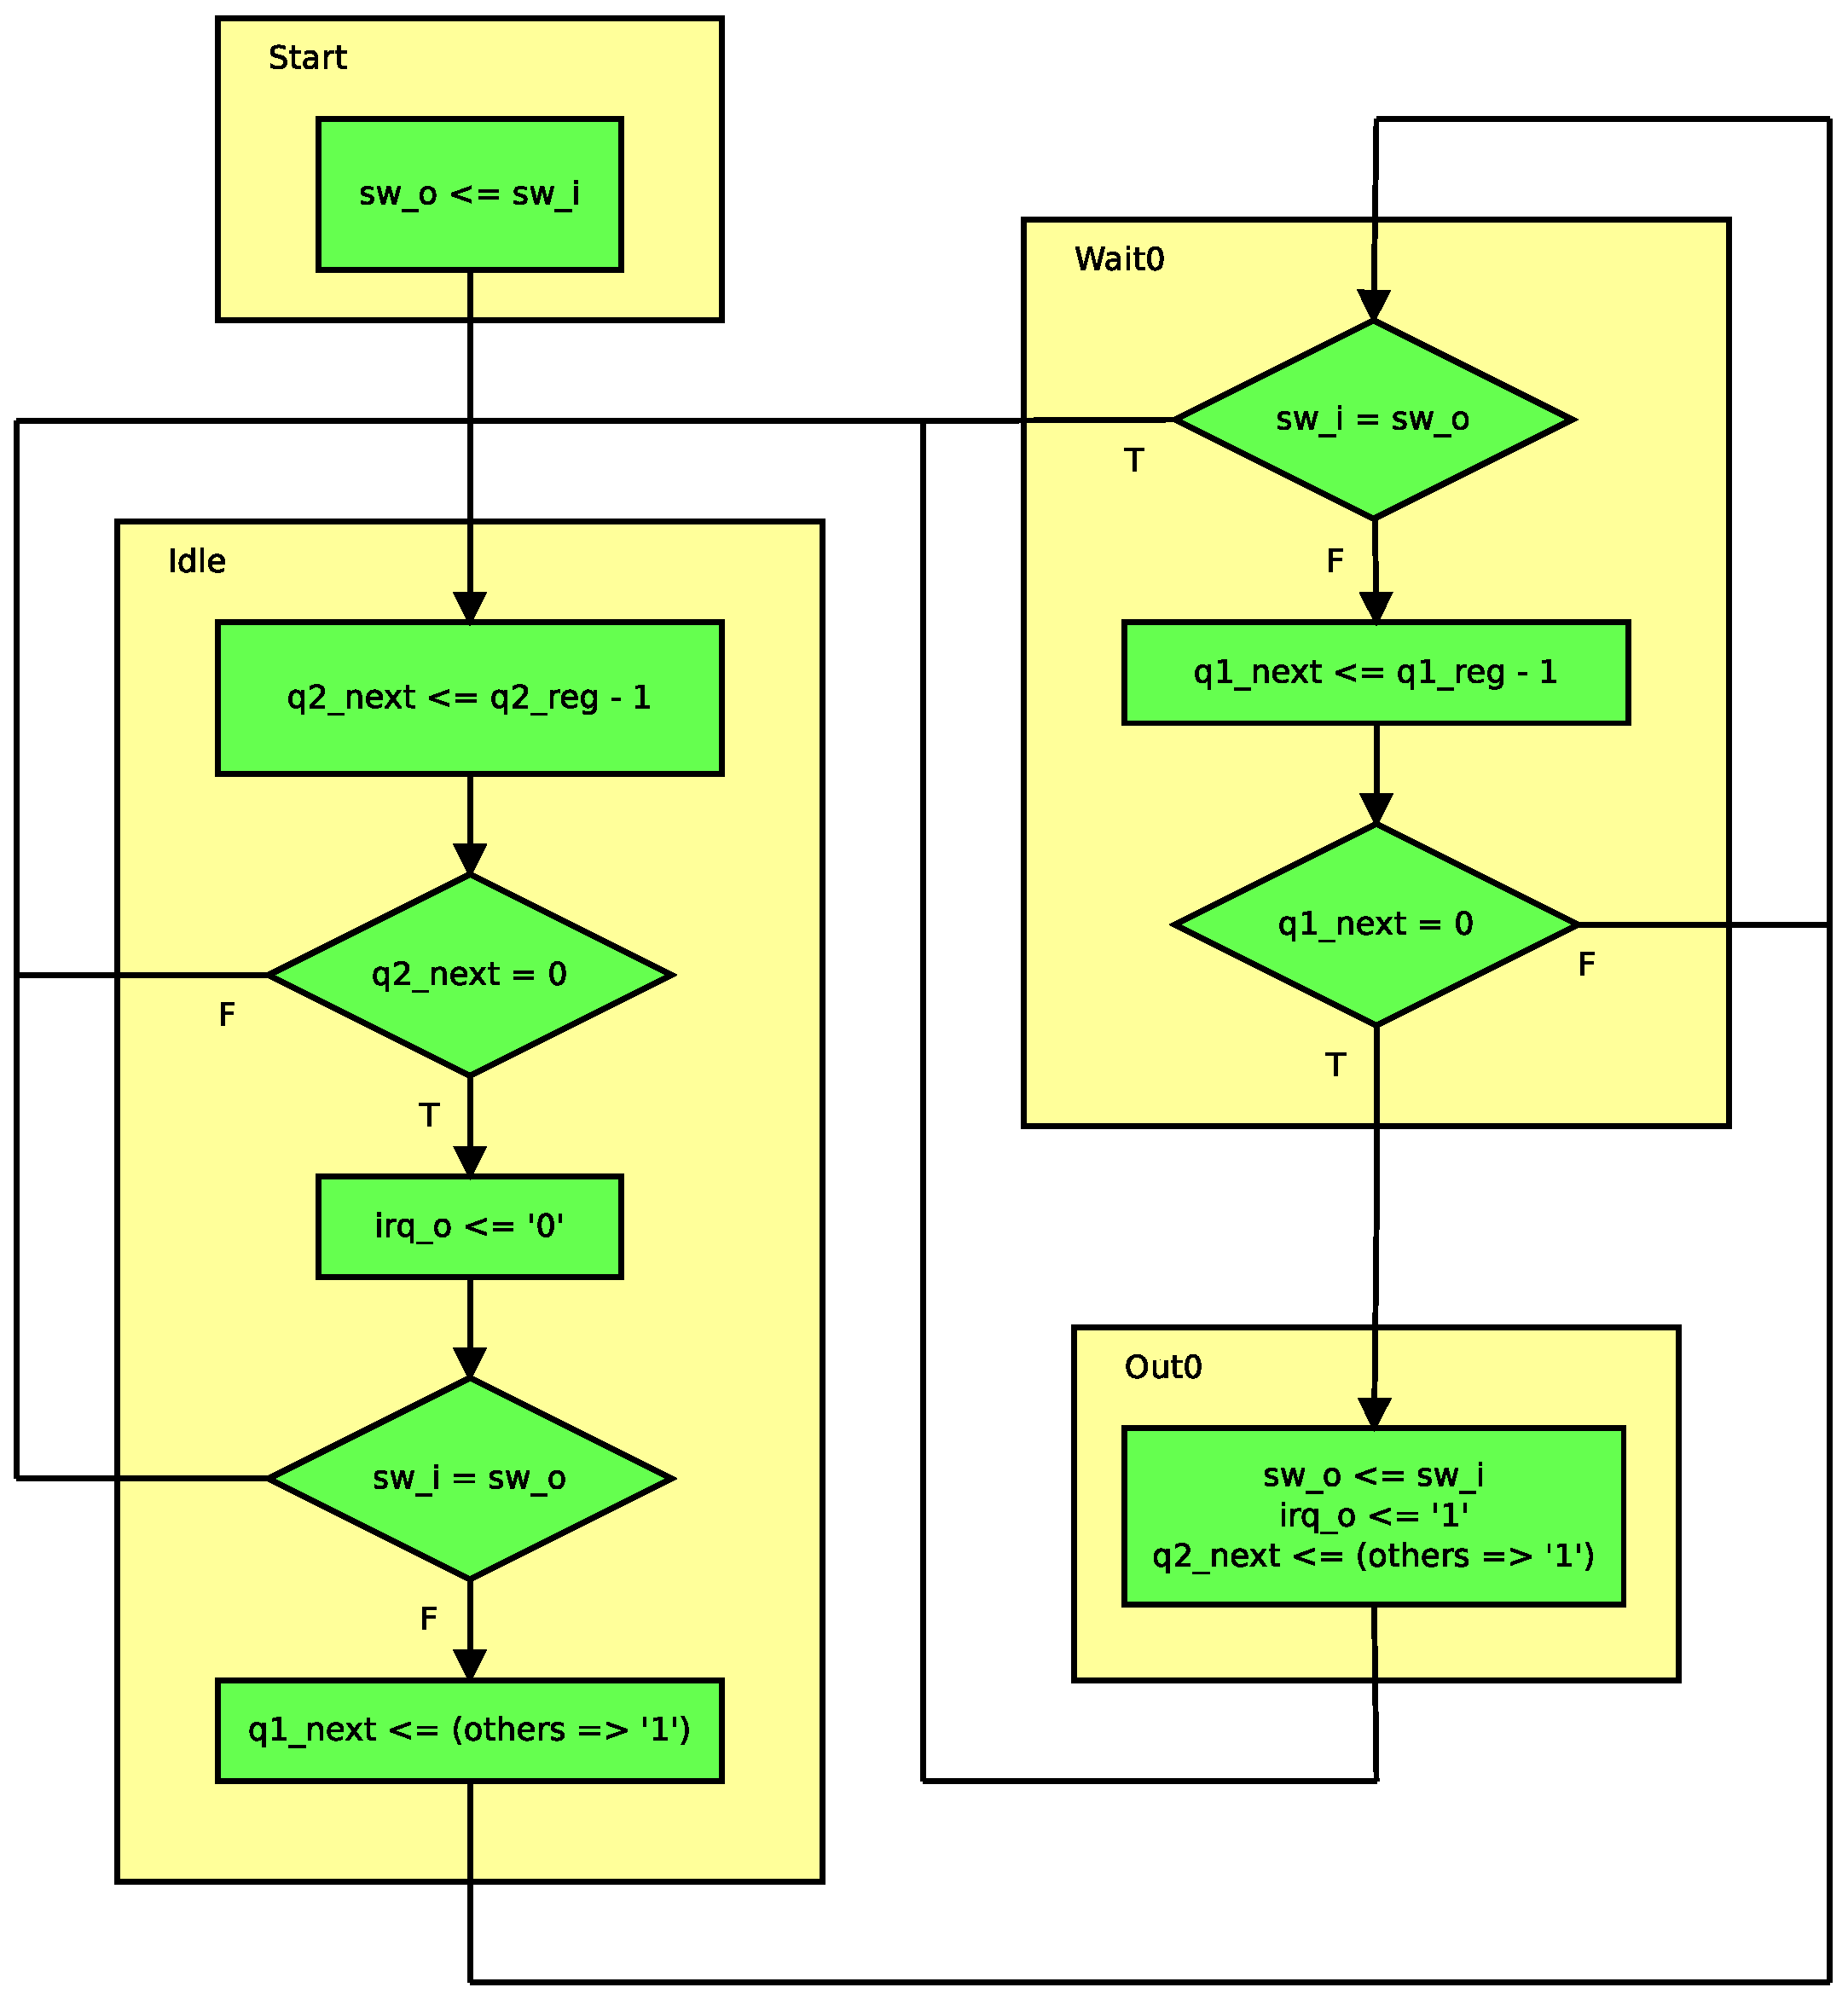
\includegraphics[width=0.7\textwidth]{images/tb6_switch_FSD.eps}
		\caption{Switch block state machine}
	\end{centering}
\end{figure}

\subsubsection{Implementation}
%     	   Implementation
%
%                Mechanical drawings with details explained
%                Electronic diagrams with details explained
%                Source code with details explained
%                Description of integration 
%
The code for the IDLE state is shown below, here the "q2" delay is used in the start, then the interrupt pin is set to zero, then the input and output is compared, if they are not equal the next state is WAIT0 and the "q1" delay is set.
\begin{lstlisting}[language=VHDL]
...
when IDLE =>
	q2_next <= q2_reg-1;
	if	(q2_next = 0) then
		irq_o <= '0';
		if	(sw_i = sw_o) then
			state_next <= IDLE;
		else
			q1_next		<= (others => '1');
			state_next	<= WAIT0;
		end if;
	else
		state_next <= IDLE;
	end if;
...
\end{lstlisting}
In the WAIT0 state the input and output is compared repeatedly to check if the input is stable. If the input is stable long enough time the OUT0 state is entered.
\begin{lstlisting}[language=VHDL]
...
when WAIT0 =>
	if	(sw_i = sw_o) then
		state_next <= IDLE;
	else
		q1_next <= q1_reg-1;
		if	(q1_next = 0) then
			state_next <= OUT0;
		else
			state_next <= WAIT0;
		end if;
	end if;
...
\end{lstlisting}
In the OUT0 state the switch output is set to switch input signal, and an interrupt signal is set high, the "q2" delay is set and it returns to the IDLE state.
\begin{lstlisting}[language=VHDL]
...
when OUT0 =>
	sw_o		<= sw_i;
	irq_o		<= '1';
	q2_next		<= (others => '1');
	state_next	<= IDLE;
...
\end{lstlisting}

\subsubsection{Verification}
%       	 Verification
%
%                Module tests
%                Integration tests
%                Acceptance test
The code is tested on a test bench in isim. The test verify that the block first set the switch output after the input has been stable for a while. And when the output is set the interrupt signal is set high for some time and then set low again. 
\begin{figure}[H]
	\begin{centering}
		%\missingfigure{Updated timebox figure}
		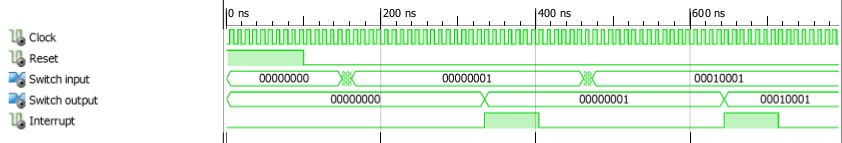
\includegraphics[width=1.0\textwidth]{images/tb6_switch_tb.png}
		\caption{Switch block test bench}
	\end{centering}
\end{figure}
\subsubsection{Conclusion}
% % % % % % % % % % % % % % % % % % % % % % % % % % % % % % % % % % % % % % % % %
% % % % % % % % % % % % % % % % % % % % % % % % % % % % % % % % % % % % % % % % %
% Jesus Thing
% % % % % % % % % % % % % % % % % % % % % % % % % % % % % % % % % % % % % % % % %
\subsection{WebServer - Paulo}
%			Intro
%					verification specification
%					deployment specification
%
In time box 4 a web server was implemented at the ip address 10.1.18.223, this is a virtual machine assign as development environment for the uClinux distribution. The server is running Apache 2, PHP version 5.1.6 and MySQL server 5.0.95.
In this time box a web services system is developed for the communication between the Embedded device and the web server and the other way around. The web page made in Project 3 is incorporated with server side scripts for a fully functional web interface.
\subsubsection{Analysis}
%			Analysis
%
%                Refactored block diagram
%                Refactored class diagram
%                Detailed use cases
%                User interface specification
%                System interface specification
%                Dimensioning specification 
%
For a fully functional web interface the communication have to present in both direction since some teams need to send commands from them web page to the modules.
For the fully cooperation with all the teams a file structure was created in the server, where each team have is own folder where all the needed scripts, images and layout styles can be implemented without changing the main layout approved in project 3.
\lineparagraph{Web interface file Structure}
\begin{itemize}
	\item index.php
	\item savedata.php
	\item sendcmd.php
	\item saveip.php
	\item ajax.js
	\item login.php 
	\item cron.php 
	\item includes\/ 
	\begin{itemize}
		\item db\_connect.php
		\item db\_globals.php
	\end{itemize} 
	\item modules\/ 
		\begin{itemize}
		\item photovoltaic\/ 
			\begin{itemize}
				\item index.php
				\item db\_connect.php
				\item cron.php 
				\item (Each team choose the rest of the scripts) 
			\end{itemize}
		\item caes\/ 
			\begin{itemize}
				\item index.php 
				\item db\_connect.php 
				\item cron.php 
				\item (Each team choose the rest of the scripts) 
			\end{itemize}
		\item hub\/
			\begin{itemize} 
				\item index.php 
				\item db\_connect.php 
				\item cron.php 
				\item (Each team choose the rest of the scripts) 
			\end{itemize}
		\item battery\/ 
			\begin{itemize}
				\item index.php 
				\item db\_connect.php 
				\item cron.php 
				\item (Each team choose the rest of the scripts) 
			\end{itemize}
		\item windturbine\/ 
			\begin{itemize}
				\item index.php 
				\item db\_connect.php 
				\item cron.php 
				\item (Each team choose the rest of the scripts)
			\end{itemize}
	\end{itemize}
\end{itemize}

A short description for each script can be seen bellow:
\begin{itemize}
	\item index.php - First page of the web interface.
	\item savedata.php - Webservice that save data retrieved from the module to the database.
	\item sendcmd.php - Webservice to send commands to the desired module in the system.
	\item saveip.php - Webservice necessary to save the ip address of the energy hub, this will keep the system up and running even if a change on the network is made.
	\item ajax.js - This Javascript handle AJAX requests when the page have no need to be reloaded, that ensure less bandwidth in the web server.
	\item login.php  - This PHP script makes the authentication of the user, creating a session when the user gives the right certifications.
	\item cron.php  - Cron jobs are running by the server in a predefined time, in this case the cron.php at the web server root will point to the cron jobs inside each module folder.
	\item db\_connect.php - Handle the connection to the MySQL database.
	\item db\_globals.php - Includes all the global variables with the credentials for the database.
\end{itemize}

\lineparagraph{Communication}
The server have to be able to save the data retrieved from the system and send commands to the the modules connected to the energy hub. Web services are created for this functionalities.

Bellow we have the flow of the communication from the user until the final destination in this case the module or the energy hub.
\begin{figure}[H]
	\begin{centering}
		\missingfigure{Communication SendCmd.php}
		%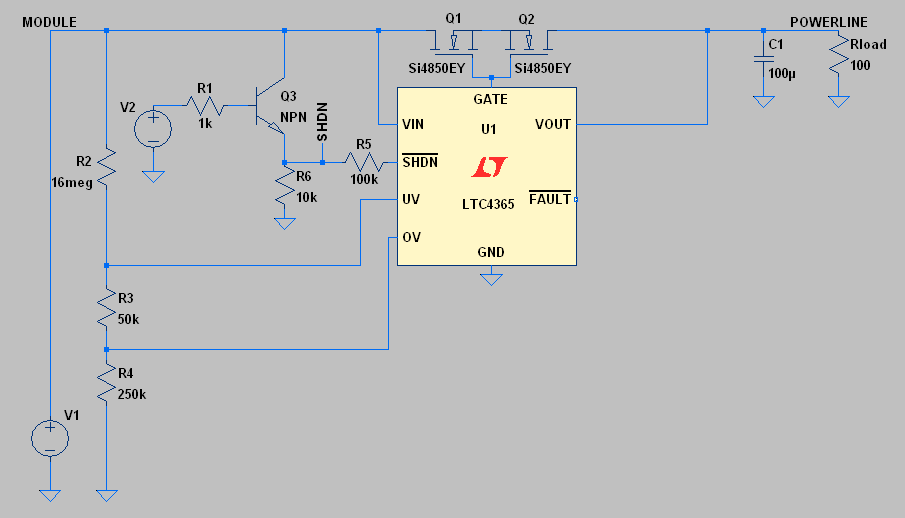
\includegraphics[width=1\textwidth]{images/tb5_LTC_simu1.png}
		%\caption{Schematics for the device LTC4365}
	\end{centering}
\end{figure}

This script doesn't give any feedback to the user, the commands send are not verified by the web server or the energy hub. The commands are handle by each module. With this system the flexibility of the system is ensured, since new modules can be added with different functionalities from the already known.
An application running in background at the energy hub uClinux, ensure that the command is translated to UART so it can be send through the power line communication to the modules.
\\\\
Measurements to be saved in the database:
\begin{figure}[H]
	\begin{centering}
		\missingfigure{Communication SendCmd.php}
		%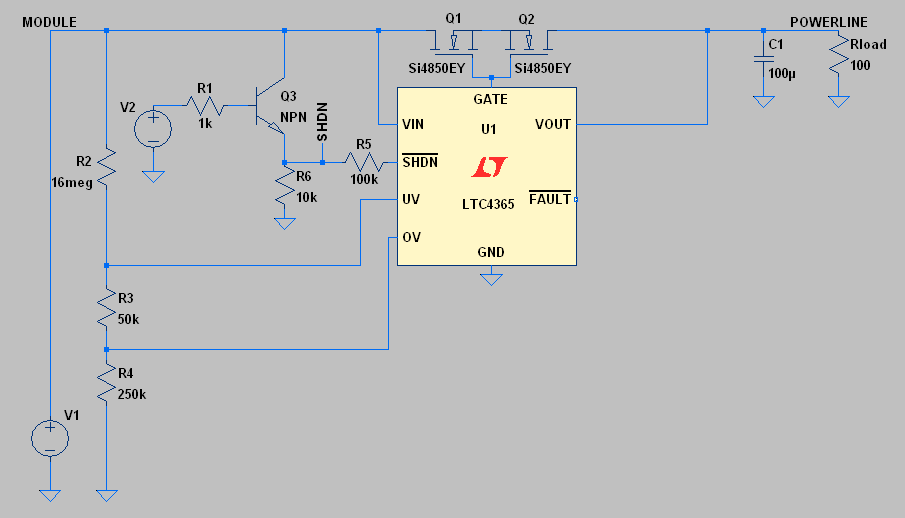
\includegraphics[width=1\textwidth]{images/tb5_LTC_simu1.png}
		%\caption{Schematics for the device LTC4365}
	\end{centering}
\end{figure}
To retrieve the measurements from the modules, an application running at the energy hub translate the data retrieved from the module through PLC to a URL request at the web server. In the server side the web server will collect the data and save it in the database.
\\\\
IP address is send from the Embedded Device:
\begin{figure}[H]
	\begin{centering}
		\missingfigure{Communication SendCmd.php}
		%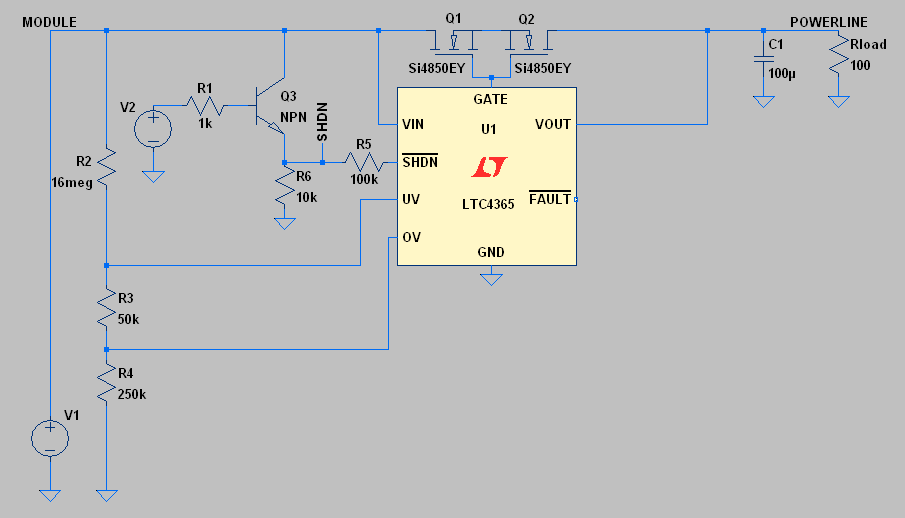
\includegraphics[width=1\textwidth]{images/tb5_LTC_simu1.png}
		%\caption{Schematics for the device LTC4365}
	\end{centering}
\end{figure}
A background application running at the uClinux, ensure that after reset the system IP address assigned by DHCP to the energy hub is saved in the database so commands can be send through the web interface. This add flexibility to the system, since a change in the network could stop the normal work of the system.

\subsubsection{Design}
%       	 Design
%
%                UML/SysML deployment view(s)
%                Mechanical specifications and dimensioning
%                HW module specification per block
%                UML SW deployment view
%                Class specification
%                Refactored class diagram
%                Use case scenarios specifications
%                Sequence diagrams
%
\subsubsection{Implementation}
%     	   Implementation
%
%                Mechanical drawings with details explained
%                Electronic diagrams with details explained
%                Source code with details explained
%                Description of integration 
%
\subsubsection{Verification}
%       	 Verification
%
%                Module tests
%                Integration tests
%                Acceptance test
\subsubsection{Conclusion}
% % % % % % % % % % % % % % % % % % % % % % % % % % % % % % % % % % % % % % % % %
% % % % % % % % % % % % % % % % % % % % % % % % % % % % % % % % % % % % % % % % %
% Dennis Thing
% % % % % % % % % % % % % % % % % % % % % % % % % % % % % % % % % % % % % % % % %
\subsection{UART Device driver improvements - Dennis}
As described in section \ref{sec:device_driver_conclusion}, some improvements should be implemented in order to boost performance on the UART devices. The parts which will be further implemented in the UART device driver is:
\begin{itemize}
	\item Interrupt controlled read.
	\item More flexibel initialization. 
	\item Better feedback/help description to the user. 
\end{itemize}
Furthermore it was pointed out (by Klaus Kolle) that the implemented way of setting up the device broke general politic for device drivers. To avoid this, an IOCTL (Input Output Control) function shall be implemented to take care of all setup and to leave the write function to sending characters. 
%			Intro
%					verification specification
%					deployment specification
%
%\subsubsection{Analysis}
%			Analysis
%
%                Refactored block diagram
%                Refactored class diagram
%                Detailed use cases
%                User interface specification
%                System interface specification
%                Dimensioning specification 
%
\subsubsection{Design}
The functionalities implemented in the IOCTL call are:
\begin{itemize}
	\item Help command. Write out the different choices of IOCTL calls.
	\item Default setup call. Sets up the defined UART to 8n1, 9600 baud rate. 
	\item Baud rate. Set a baud rate in the range 2400 to 230400.
	\item Word length. Define the word length between 5 and 8.
	\item Stop bits. Number of stop bits, 1 or 2.
	\item Parity bits. Define parity bit setting: none, odd, even, forced 1 stick, forced 0 stick.
	\item Fifo. Enable or disable fifo.
	\item Fifo trigger. Number of characters in the buffer before an interrupt: 1,4,8,14
\end{itemize}

%       	 Design
%
%                UML/SysML deployment view(s)
%                Mechanical specifications and dimensioning
%                HW module specification per block
%                UML SW deployment view
%                Class specification
%                Refactored class diagram
%                Use case scenarios specifications
%                Sequence diagrams
%
\subsubsection{Implementation}
Common header file for the UART device driver and the UART user space application. The magic number 'k' is used to by the IOCTL macros \_IO and \_IOR to create an IOCTL number, which is then decoded and verified in the kernel module. 
\begin{lstlisting}[language=c]
#ifndef UARTIOCTL_H
#define UARTIOCTL_H

#include <linux/ioctl.h>

#define UART_IOC_MAGIC  'K'

#define IOCTL_HELP 		_IO(UART_IOC_MAGIC,  1)
#define IOCTL_DEFAULT	_IO(UART_IOC_MAGIC,  2)
#define IOCTL_BAUD 		_IOR(UART_IOC_MAGIC, 3, int)
#define IOCTL_WORDLEN 	_IOR(UART_IOC_MAGIC, 4, int)
#define IOCTL_STOPBIT 		_IOR(UART_IOC_MAGIC, 5, int)
#define IOCTL_PARBIT 		_IOR(UART_IOC_MAGIC, 6, int)
#define IOCTL_FIFO			_IOR(UART_IOC_MAGIC, 7, int)
#define IOCTL_FIFO_TRIG 	_IOR(UART_IOC_MAGIC, 8, int)

#define UART_IOC_MAXNR 8

#endif
\end{lstlisting}

Using IOCTL to setup UART registers. Note that the \textit{fwrite} call cannot be used with IOTCL, as it needs an file descriptor instead of a file pointer. Therefore the libraries \textit{fcntl.h} and \textit{unistd.h} are included in order to use the functions \textit{open, close, read, write} and \textit{ioctl} as they make use of the file descriptor. 
\begin{lstlisting}[language=c]
	if(strncmp("io", argv[1], 2) == 0){
		if ((fd = open(UART,O_RDWR)) < 0){
     	          	printf("Cannot open file.\n");
			exit(-1);
        	}

		ret_val = ioctl(fd, IOCTL_DEFAULT);
		if(ret_val < 0){
			printf("ioctl_get_msg failed:%d\n", ret_val);
			exit(-1);
		}
		ret_val = ioctl(fd, IOCTL_BAUD, 19200);
		if(ret_val < 0){
			printf("ioctl_get_msg failed:%d\n", ret_val);
			exit(-1);
		}

		close(fd);
	}
\end{lstlisting}
Loop reading used for testing purpose of the power line communication. 
\begin{lstlisting}[language=c]
	---
	else if(strncmp("readloop", argv[1], 8) == 0){
		if ((fd = open(UART,O_RDONLY)) < 0){		//Open the file
     	          	printf("Cannot open file.\n");
			exit(-1);
        	}
		while(1){
			if(read(fd,rb,10) != 0) 
				printf("%s\n",rb);
		}
		printf("\n");
		close(fd);
	}
\end{lstlisting}

IOCTL added to file operator
\begin{lstlisting}[language=c]
static struct file_operations uart_fops = {
	.owner   	= THIS_MODULE,
	.read			= uart_read,
	.write  	= uart_write,
	.open    	= uart_open,
	.ioctl	 	= uart_ioctl,
	.release 	= uart_close,
};
\end{lstlisting}

IOCTL implementation. At first the function verifies the IOCTL number sent and checks if the transferred command is valid. The rest of the function is a  switch/case which takes the cmd parameter sent and performs an action according to the command (help, default setup, baud rate etc.)
\begin{lstlisting}[language=c]
/******************************************************************************
 * IOCTL call
 *****************************************************************************/
static int uart_ioctl(struct inode *inode, struct file *filp, unsigned int cmd, unsigned long arg){
	unsigned int num = 0;
        int err = 0, ret = 0;
	int div, mult,bflag = 0;
	unsigned int baud = 0;

        /* don't even decode wrong cmds: better returning  ENOTTY than EFAULT */
        if (_IOC_TYPE(cmd) != UART_IOC_MAGIC) return -ENOTTY;
        if (_IOC_NR(cmd) > UART_IOC_MAXNR) return -ENOTTY;

        /*
         * the type is a bitmask, and VERIFY_WRITE catches R/W
         * transfers. Note that the type is user-oriented, while
         * verify_area is kernel-oriented, so the concept of "read" and
         * "write" is reversed
         */
        if (_IOC_DIR(cmd) & _IOC_READ) err = !access_ok(VERIFY_WRITE, (void __user *)arg, _IOC_SIZE(cmd));
        else if (_IOC_DIR(cmd) & _IOC_WRITE) err =  !access_ok(VERIFY_READ, (void __user *)arg, _IOC_SIZE(cmd));
        if (err) return -EFAULT;
	// Get minor number
	num = MINOR(inode->i_rdev);
	DPRINT("\nuart%d_ioctl, ioctl_cmd: %u\n",num,cmd);
	// Check if minor number is okay
	if(num >= NUM_UART_DEVICES){
		return -ENODEV;
	}

	switch (cmd) {
	/***************************** HELP ************************************************/
	case IOCTL_HELP:
	    DPRINT("\nHELP\n");
	    help();	// Print different IOCTL call options to user
	  break;
	/***************************** DEFAULT *********************************************/
	case IOCTL_DEFAULT:
	    m_reg_write(ulcr[num], 0x80);	// Enable write to divisor latch
	    m_reg_write(udll[num], (unsigned char)((LPC24xx_Fpclk/(16*9600)) & 0xFF));
	    m_reg_write(udlm[num], (unsigned char)((LPC24xx_Fpclk/(16*9600)) >> 8));
	    m_reg_write(ulcr[num], 0x03);	// 8N1 setup and disable write to divisor latch
	    m_reg_write(ufcr[num], 0x7);	// Enable FIFO's
	  break;
	/***************************** BAUD ************************************************/
	case IOCTL_BAUD:
	    if(arg < 2400 || arg > 230400){	// Verify argument
		printk("\nInvalid parameter");
		return -EFAULT;
	    }
	    bflag = 0;	
	/* From datasheet:
	   Mult values: 1-15, Div: 0-14. Mult shall be bigger than div.
	   DLL shall be above 2 if DLM is zero.

	*/ 
	   // Loop through different div and mult values in order to get a integer value to
	   // the divisor latch reg (DLM+DLL).
	    for(div = 0; div <= 15; div++){
		for(mult = div+1; mult <= 15; mult++){
		    baud = ((16*arg)+((16*arg*div)/mult));
		    if(LPC24xx_Fpclk%baud == 0){
			if((div != 0) && ((LPC24xx_Fpclk/baud) >= 3)){
			    bflag = 1;
			    break;
			}
		    }
		}
		if(bflag==1) break;
	    }
	    DPRINT("\ndiv: %d, mult: %d, baud: %d",div,mult,baud);
	    if(div == 15){	// If no value was found, return error
		printk("\nCannot calculate BAUD!");
		return -EFAULT;
	    }
	    m_reg_bfs(ulcr[num], 0x80); // Enable write to divisor latch
	    m_reg_write(ufdr[num], ((div<<0) | (mult<<4)));	// Write div and mult to fraction dividor reg
	    m_reg_write(udll[num], (unsigned char)((LPC24xx_Fpclk/baud) & 0xFF)); // Input DLL val (8 lowest bits)
	    m_reg_write(udlm[num], (unsigned char)((LPC24xx_Fpclk/baud) >> 8));	  // Input DLM val (8 highest bits)
	    m_reg_bfc(ulcr[num], 0x80);	// Disable write to divisor latch

	  break;
	/***************************** Wordlen *********************************************/
	case IOCTL_WORDLEN:
	    if(arg < 5 || arg > 8){	// Verify that argument is valid
		printk("\nInvalid parameter");
		return -EFAULT;
	    }
	    m_reg_bfc(ulcr[num], 0x3);	// Clear bits holding world lenght
	    m_reg_bfs(ulcr[num], ((arg-5)<<0));	// Inset value for world lenght
	  break;
	/***************************** STOP bits *******************************************/
	case IOCTL_STOPBIT:
	    if(arg != 1 || arg != 2){	// Verify that argument is valid
		printk("\nInvalid parameter");
		return -EFAULT;
	    }
	    m_reg_bfc(ulcr[num], (1<<2)); // Set stop bit to 1
	    if(arg == 2){
	    	m_reg_bfs(ulcr[num], (1<<2)); // Set stop bit to 2
	    }
	  break;
	/***************************** Parity Bit ******************************************/
	case IOCTL_PARBIT:	
	    if(arg < 0 || arg > 4){ // Verify that argument is valid
		printk("\nInvalid parameter");
		return -EFAULT;
	    }
	    m_reg_bfc(ulcr[num], (1<<3));	// Disable parity bits. if 0 was written
	    if(arg > 0){
		m_reg_bfs(ulcr[num], (1<<3));	// Enable parity.
		m_reg_bfs(ulcr[num], ((arg-1)<<4)); // Set parity (odd, even, forced 0 or 1
	    }
	  break;
	/***************************** FIFO Enable *****************************************/
	case IOCTL_FIFO:
	    if(arg != 0 || arg != 1){ // Verify that argument is valid
		printk("\nInvalid parameter");
		return -EFAULT;
	    }
	    m_reg_bfc(ufcr[num], 0x7);	// Disable fifo
	    if(arg==1){
		m_reg_bfs(ufcr[num], 0x7);	// Enable fifo
	    }
	  break;	
	/***************************** FIFO Enable *****************************************/
	case IOCTL_FIFO_TRIG:
	    if(arg != 1 || arg != 4 || arg != 8 || arg != 14){	// Verify that argyment is valid
		printk("\nInvalid parameter");
		return -EFAULT;
	    }
	    m_reg_bfc(ufcr[num], 0xC0);	// Clear bits holding trigger level
	    m_reg_bfs(ufcr[num], (int)((arg/4)<<6));	// 1/4=0, 4/4=1, 8/4=2, 14/4=3
	  break;	
	/***************************** Wrong ***********************************************/
	default:
	    help();	// If wrong parameter sent. Print options. 
	    return -ENOTTY;
	}

        return ret;
}
\end{lstlisting}

Interrupt implementation. The interrupt is requested in the open call. If there is no data to read, the module is sent to sleep and awaken again when the buffer is not empty anymore. In close the interrupt is freed again. 
\begin{lstlisting}[language=c]
//Interrupt sources for UART0,1,2,3
#define UART0_IRQ 6 
#define UART1_IRQ 7
#define UART2_IRQ 28
#define UART3_IRQ 29
//Array of interrupt flags
static int flag[NUM_UART_DEVICES];

//Prototypes of interrupt functions. Int\_uart is an array of function pointers.
static irqreturn_t interrupt_uart0(int irq, void *dev_id);
static irqreturn_t interrupt_uart1(int irq, void *dev_id);
static irqreturn_t interrupt_uart2(int irq, void *dev_id);
static irqreturn_t interrupt_uart3(int irq, void *dev_id);
typedef irqreturn_t (*INTERRUPT_UART)(int irq, void *dev_id);
const INTERRUPT_UART int_uart[NUM_UART_DEVICES] = {interrupt_uart0, interrupt_uart1, interrupt_uart2, interrupt_uart3};

static int uart_open(struct inode* inode, struct file* file){
---
	flag[num] = 0;
	m_reg_write(uier[num], 0x1);	//Enable interrupt on rx buf not empty
	m_reg_bfs(VICSoftIntClear, (1<<uirq[num])); // Clear interrupts from uart source
	m_reg_bfs(VICIntEnable, (1<<uirq[num]));    // Enable uart interrupt

	ret = request_irq(uirq[num], int_uart[num], SA_INTERRUPT,"UART interrupt", NULL); //NULL = Pointer based on IRC handler

	if(ret){
		printk("IRQ %d is not free. RET: %d\n", UART2_IRQ,ret);
		return ret;
	}
	return 0;
}

static int uart_close(struct inode* inode, struct file* file){
	---
	free_irq(uirq[num], NULL);	// Free interrupt
	return 0;
}
\end{lstlisting}
UART read call.
\begin{lstlisting}[language=c]
static ssize_t uart_read(struct file *p_file, char *p_buf, size_t count, loff_t *p_pos){
	---
	if(!(m_reg_read(ulsr[num]) & 0x01)){		//If the read buffer is empty, go to sleep.
		DPRINT("\nBUF EMPT, SLEEP\n");
		wait_event_interruptible(my_queue, (flag[num] != 0));	// Put the function to sleep
		flag[num] = 0;
	}
	else{
		cread = m_reg_read(urbr[2]);
	}
	*p_buf = cread;		// Write value to read buffer. 
	
	return count;
}
\end{lstlisting}
UART interrupt function. The four different interrupt functions are all similar, except for the registers that is handled. 
\begin{lstlisting}[language=c]
/******************************************************************************
 * Interrupt recieve routine UART2
 *****************************************************************************/
static irqreturn_t interrupt_uart2(int irq, void *dev_id){
	
	cread = m_reg_read(urbr[2]);		// Read the buffer
	
	DPRINT("\nREAD VAL: %c\n", cread);		

	m_reg_bfs(VICSoftIntClear, (1<<uirq[2]));		// Clear int flag in vic
	flag[2] = 1;	
	wake_up_interruptible(&my_queue);		// Wake up from interrupt
	return IRQ_HANDLED;
}
\end{lstlisting}

The help function implemented gives the following input if it is called:
\begin{lstlisting}[language=c]
# ./uart help
Available commands:
  IOCTL_HELP : show different help commands
  IOCTL_DEFAULT : 8N1, 9600 baud
  IOCTL_BAUD : send argument between 2400 and 230400
  IOCTL_WORDLEN : send argument 5-8 wordlenght
  IOCTL_STOPBIT : send argument, 1 or 2 stop bits
  IOCTL_PARBIT : send arg, 0, 1(odd), 2(even), 3(Forced 1 stick), 4(Forced 0 stick
  IOCTL_FIFO : send arg 0 (off), 1 (on)
  IOCTL_FIFO_TRIG : send arg number to trig, 1, 4, 8 or 14 characters
\end{lstlisting}

\subsubsection{Verification}
According to the requirement F-1.2 and the test for it, the communication between two modules have been tested over power line. 
\begin{table}[H]
\centering
	\begin{tabular}{|p{1.2cm}|p{2.3cm}|p{9.5cm}|p{2.5cm}|}
	\hline
	ID		& Requirement		& Test Description		& Grade/Comment\\\hline
	F-1.2		& Communication - System & Connect a module to the hub, by connecting the module to the hubs power line (plugs on the back of the hub). If the module respond to a ping signal send from the hub, the two modules are communicating through power line. The response of the ping can be seen by using an oscilloscope and simply analyzing the packages on the power line according to the protocol. & PASSED\\\hline
	\end{tabular}
\end{table}
A small test setup have been made with a MBED device as one of the modules and an ARM board running uClinux as the other module. Data have been sent in both direction (from the MBED to the ARM and from the ARM to the MBED) through each of their Power Line modules, with use of the UART user space application written. The default settings of the Power Line module is 8N1 with a baud rate of 19200 which has been used for the test. 
\\ The test has passed. No invalid or missing data have been observed throughout the test. 
%       	 Verification
%
%                Module tests
%                Integration tests
%                Acceptance test
\subsubsection{Conclusion}
The UART module is working with implemented IOCTL and interrupt handler.
Further improvements before the fully functional energy system can use the UART driver is implementation of file write.
% % % % % % % % % % % % % % % % % % % % % % % % % % % % % % % % % % % % % % % % %
% % % % % % % % % % % % % % % % % % % % % % % % % % % % % % % % % % % % % % % % %
% Deployment
% % % % % % % % % % % % % % % % % % % % % % % % % % % % % % % % % % % % % % % % %
\subsection{Deployment}
	%which versions of the prototype the customer will get
	%with what functionality.
\paragraph{Theis thing}
%
%
\paragraph{Jesus thing}
%
%
\paragraph{Dennis thing}
%
%